\documentclass[11pt,letterpaper]{article}
\usepackage[margin=0.93in]{geometry}
\usepackage[T1]{fontenc}
\usepackage{lmodern}
\usepackage{microtype}
\usepackage{amsmath,amssymb,mathtools,amsthm}
\usepackage{booktabs}
\usepackage{enumitem}
\usepackage{xcolor}
\usepackage{hyperref}
\usepackage{tikz}
\usetikzlibrary{arrows.meta,positioning}
\hypersetup{colorlinks=true,linkcolor=blue!50!black,urlcolor=blue!50!black,pdftitle={High-Order Co-normal Flux Correction in Jacobi-Simplex HPS}}
\setlist[itemize]{leftmargin=1.35em,itemsep=2pt,topsep=4pt}
\setlist[enumerate]{leftmargin=1.55em,itemsep=3pt,topsep=4pt}
\allowdisplaybreaks[1]
\newcommand{\RR}{\mathbb R}
\newcommand{\PP}{\mathcal P}
\newcommand{\Tau}{\mathcal T}
\newcommand{\lam}{\boldsymbol\lambda}
\newcommand{\gam}{\boldsymbol\gamma}
\newcommand{\muh}{\widehat{\boldsymbol\mu}}
\newcommand{\fint}{\mathbf f^{\mathrm{int}}}
\newcommand{\qlow}{\mathbf q_L}
\newcommand{\qhigh}{\mathbf q_H}
\newcommand{\bb}{\mathbf b}
\newcommand{\zz}{\mathbf z}
\newcommand{\gvec}{\mathbf g}
\newcommand{\cc}{\mathbf c}
\title{High-Order Co-normal Flux Correction\\[3pt]
\large Variable Robin Boundary Conditions in Dense Jacobi-Simplex HPS}
\author{Technical derivation and implementation note - Sachin Natesh}
\date{11 October 2026}
\begin{document}
\maketitle
\vspace{-1.3em}
\begin{abstract}
The existing hierarchical Poincar\'{e}--Steklov (HPS) skeleton carries degree-\(n\) face traces and a degree-\(n\) \emph{tau-stabilized numerical co-normal flux}. For polynomial diffusion of degree \(p_A\ge2\), the physical co-normal flux of a degree-\(n\) volume solution can have degree greater than \(n\). A spatially varying Robin coefficient \(\beta\) can couple these omitted high modes back into the degree-\(n\) boundary equations. We derive a correction that observes the physical high flux on true exterior faces, propagates its affine dependence through existing HPS interface reconstruction maps, and modifies only the root Robin operator and right-hand side. Neither the degree-\(n\) interface skeleton nor its tau-stabilized merge equations is enlarged. The current intended implementation is \textbf{Dense-only}; DenseSparse, MatrixFree, and Verify remain outside this extension.
\end{abstract}

\section{Equation, approximation spaces, and the missing information}
Consider a conforming affine simplicial mesh in dimension \(D\), and the divergence-form equation
\begin{equation}\label{eq:pde}
 -\nabla\!\cdot\!\bigl(A(x)\nabla u\bigr)+b(x)\cdot\nabla u+c(x)u=f(x),
\end{equation}
with Robin data on the physical exterior boundary \(\partial\Omega\):
\begin{equation}\label{eq:robin}
 \alpha(x)u(x)+\beta(x)q(x)=g(x),\qquad
 q=n_{\mathrm{out}}^{T}A(x)\nabla u(x).
\end{equation}
On each element \(K\), approximate \(u\) by degree-\(n\) volume Jacobi polynomials. The \(\kappa\)-weighted volume basis and its residual family \(\kappa_{\mathrm{res}}=\kappa+\mathbf 2\) follow the existing implementation convention. The divergence-form coefficient adapter forms
\begin{equation}\label{eq:expanded}
 \widetilde A_{rs}=-A_{rs},\qquad
 \widetilde b_s=b_s-\sum_{r=1}^{D}\partial_{x_r}A_{rs},\qquad
 \widetilde c=c,
\end{equation}
then promotes the coefficients to \(\kappa_{\mathrm{res}}\). The expanded interior operator is unchanged. As the existing leaf convention is \(L\cc=-\fint\), input physical source moments use \(\fint=-\mathbf f_{\mathrm{phys}}\). This sign convention does not alter any of the flux formulas below.

Every face uses the \emph{same canonical} degree-\(n\) Jacobi face basis, with face family given by the first \(D\) entries of the volume parameter vector. Put
\begin{equation}
 V_L=\Pi_n^{D-1},\qquad k_L=\dim V_L.
\end{equation}
Let \(\PP_L\) denote the weighted face-moment projection onto \(V_L\). For a degree-\(p_A\) diffusion tensor,
\begin{equation}\label{eq:qdegree}
 u|_K\in\Pi_n^D\quad\Longrightarrow\quad
 q|_f\in\Pi_{p_H}^{D-1},\qquad p_H=n+p_A-1
\end{equation}
(as an upper bound). We split the face coefficient vector of the \emph{physical} flux into low degrees \(0{:}n\) and high degrees \(n+1{:}p_H\):
\begin{equation}\label{eq:split}
 \qlow=\PP_L q,\qquad
 \qhigh=\PP_H q,\quad
 V_H=\Pi_{p_H}^{D-1}\ominus\Pi_n^{D-1}.
\end{equation}
Here \(\ominus\) means the orthogonal difference in the common face basis. These are coefficient vectors of weighted moments; physical face measure factors are included consistently in trace/flux maps. If \(p_A\le1\), the high space is empty. For \(D=1\), a face is a point and also has no high modes.

\section{The ordinary tau-stabilized HPS leaf}
Let \(\cc_K\) be the element's volume modal coefficients and \(\lam_K\) its stacked degree-\(n\) trace degrees of freedom. Denote the interior residual, trace, and \emph{low physical co-normal flux} maps by
\begin{equation}
 L_K\cc_K,\qquad T_K\cc_K,\qquad F_{A,K}\cc_K=\mathbf q_{L,K}.
\end{equation}
The tau-stabilized least-squares system has the schematic form
\begin{equation}\label{eq:stack}
 \mathcal A_{\tau,K}\cc_K \simeq
 \begin{bmatrix}-s_{L,K}\fint_K\\ \Tau_K^{1/2}\lam_K\end{bmatrix},\qquad
 \mathcal A_{\tau,K}=
 \begin{bmatrix}s_{L,K}L_K\\ \Tau_K^{1/2}T_K\end{bmatrix},
\end{equation}
where \(\Tau_K\) is the existing (facewise degree-\(n\)) tau penalty and \(\simeq\) denotes the least-squares solve. The response maps already produced by DenseQR are
\begin{equation}\label{eq:U}
 \cc_K=U_{\lambda,K}\lam_K+U_{f,K}\fint_K,\qquad
 \begin{aligned}
 U_{\lambda,K}&=\mathcal A_{\tau,K}^{\dagger}
       \begin{bmatrix}0\\\Tau_K^{1/2}\end{bmatrix},\\
 U_{f,K}&=\mathcal A_{\tau,K}^{\dagger}
       \begin{bmatrix}-s_{L,K}I\\0\end{bmatrix}.
 \end{aligned}
\end{equation}
The skeleton uses the \emph{augmented} degree-\(n\) co-normal flux
\begin{equation}\label{eq:augflux}
 \muh_K=F_{A,K}\cc_K-\Tau_K(T_K\cc_K-\lam_K)
       =S_K\lam_K+\bb_K,
\end{equation}
with
\begin{equation}\label{eq:Sleaf}
 \boxed{\quad
 S_K=(F_{A,K}-\Tau_KT_K)U_{\lambda,K}+\Tau_K,\qquad
 G_{f,K}=(F_{A,K}-\Tau_KT_K)U_{f,K},\qquad
 \bb_K=G_{f,K}\fint_K.\quad}
\end{equation}
Here \(\bb_K\) is a \emph{source-dependent numerical-flux offset}, not the PDE advection coefficient \(b(x)\). The HPS tree stores \(S_K\) once, updates \(\bb_K\) for each source, and reconstructs \(\cc_K\) after the downward trace pass. Changing \(F_{A,K}\) does not change \(U_{\lambda,K}\) or \(U_{f,K}\).

\section{HPS interface elimination and the source upward pass}
Consider a merge of child subdomains \(A\) and \(B\). Partition each child's degree-\(n\) boundary trace into exterior-to-the-merge blocks \(E\) and the common interface block \(I\). Let \(\gam\) be the common interface trace. The children satisfy
\begin{equation}\label{eq:childflux}
 \begin{bmatrix}\muh_{A,E}\\\muh_{A,I}\end{bmatrix}
 =\begin{bmatrix}S_{A,EE}&S_{A,EI}\\S_{A,IE}&S_{A,II}\end{bmatrix}
 \begin{bmatrix}\lam_{AE}\\\gam\end{bmatrix}
 +\begin{bmatrix}\bb_{A,E}\\\bb_{A,I}\end{bmatrix},
\end{equation}
with an analogous equation for \(B\). The interface conditions are \emph{continuity of \(\gam\)} and conservation of the \emph{augmented} numerical flux,
\begin{equation}\label{eq:interface}
 \muh_{A,I}+\muh_{B,I}=0.
\end{equation}
Define the interface matrix \(K_I=S_{A,II}+S_{B,II}\). With outward co-normals on each child, the eliminated trace is
\begin{align}\label{eq:gamma}
 \gam&=R_A\lam_{AE}+R_B\lam_{BE}+\mathbf r,\\
 R_A&=-K_I^{-1}S_{A,IE},\qquad
 R_B=-K_I^{-1}S_{B,IE},\qquad
 \mathbf r=-K_I^{-1}(\bb_{A,I}+\bb_{B,I}).\nonumber
\end{align}
The parent face ordering is \([AE,BE]\). Its DtN matrix is the usual Schur-complement merge of child matrices; in particular, its source offset is
\begin{equation}\label{eq:parentb}
 \boxed{\quad
 \bb_{P,AE}=\bb_{A,E}+S_{A,EI}\mathbf r,\qquad
 \bb_{P,BE}=\bb_{B,E}+S_{B,EI}\mathbf r.\quad}
\end{equation}
The stored \(R_A,R_B\) depend only on the homogeneous child DtN matrices. The source pass refreshes \(\bb_A,\bb_B,\mathbf r,\bb_P\) without rebuilding the merge; the implementation also retains \(R_f=-K_I^{-1}\), so \(\mathbf r=R_f(\bb_{A,I}+\bb_{B,I})\). At the root, the ordinary HPS relation is
\begin{equation}\label{eq:rootdtn}
 \muh_{\mathrm{root}}=S_{\mathrm{root}}\lam_{\mathrm{root}}+\bb_{\mathrm{root}}.
\end{equation}
For \emph{constant} \(\alpha,\beta\), solve \((\alpha I+\beta S_{\mathrm{root}})\lam_{\mathrm{root}}=\gvec-\beta\bb_{\mathrm{root}}\), then reconstruct \(\gam\) downward and each \(\cc_K\) through \eqref{eq:U}. Nothing in this standard HPS procedure requires high-order skeleton unknowns.

\section{Why variable \texorpdfstring{$\beta$}{beta} needs a high-flux correction}
The degree-\(n\) root Robin equations must represent the \emph{projected product} in \eqref{eq:robin}, rather than a product of independently truncated data. The intended discrete rule (formulation B) is
\begin{equation}\label{eq:formB}
 \PP_L\bigl(\alpha\,\lam+\beta\,\widehat q_{\mathrm{full}}\bigr)=\gvec,
 \qquad \widehat q_{\mathrm{full}}=
 q_{\mathrm{physical}}-\underbrace{\Tau(T\cc-\lam)}_{\text{degree }\le n}.
\end{equation}
The penalty is already in the low numerical-flux representation \eqref{eq:augflux}. It contributes \emph{no high modes}, because the current tau weight is constant on each affine face and the trace discrepancy lies in \(\Pi_n^{D-1}\). Thus the full numerical flux is represented exactly, up to its available polynomial degree, by the pair
\begin{equation}\label{eq:fullpair}
 (\muh_L,\qhigh)\equiv
 \bigl(S_{\mathrm{root}}\lam_{\mathrm{root}}+\bb_{\mathrm{root}},\;\PP_H q_{\mathrm{physical}}\bigr).
\end{equation}
For a face polynomial \(\beta\), let \(M_\beta^{L\leftarrow L}\) and \(M_\beta^{L\leftarrow H}\) be the \emph{same weighted face multiplication operator}, with output projected to \(V_L\) and input restricted to low or high modes. If \(p_H\) is the input high cutoff, these are adjacent column blocks of
\begin{equation}\label{eq:rectM}
 M_\beta^{n\leftarrow p_H}:
 \Pi_{p_H}^{D-1}\longrightarrow\Pi_n^{D-1},\qquad
 (M_\beta)_{ij}=\int_{\widehat f}\psi_i\,\beta\,\psi_j\,w_{\kappa_{\rm face}}.
\end{equation}
The face multiplication plan and the flux moment coefficients must use the same canonical face normalization. Keeping only \(M_\beta^{L\leftarrow L}\muh_L\) discards the nonzero term \(M_\beta^{L\leftarrow H}\qhigh\).

There is a useful degree restriction. If \(\deg\beta=p_\beta\), orthogonality gives
\begin{equation}\label{eq:prune-degree}
 M_\beta^{L\leftarrow H}\psi_j=0
 \quad\text{for high input modes of degree }\deg\psi_j>n+p_\beta.
\end{equation}
Therefore only degrees
\begin{equation}\label{eq:obsdegree}
 n+1\le d\le p_{\mathrm{obs}},\qquad
 p_{\mathrm{obs}}=n+\min(p_A-1,p_\beta)
\end{equation}
need be retained for a specified \(\beta\). No high correction is needed for constant \(\beta\), \(p_A\le1\), or \(D=1\). Retaining all degrees through \(p_H\) instead is simpler and independent of subsequent updates to \(\beta\).

\section{High-order observation at a leaf}
For a globally exterior face \(f\subset\partial K\cap\partial\Omega\), construct the rectangular \emph{physical} flux moment map
\begin{equation}\label{eq:QH}
 Q_{H,K}^{f}\cc_K
 =\PP_H^f\bigl(n_f^TA\nabla u_{\cc_K}\bigr),
\end{equation}
where \(H\) selects degrees \(n+1{:}p_H\) (or the smaller relevant range \eqref{eq:obsdegree}). The map is a high-degree companion of the existing tested co-normal face map. In intrinsic canonical face coefficients, it is assembled by
\begin{equation}\label{eq:QHbuild}
 Q_{H,K}^{f}=
 \operatorname{rows}_{H}\!\left[
 J_f\sum_{s=1}^{D}
 M_{w_s^f}^{p_H\leftarrow n}\,G_s^f\right],\qquad
 w_s^f=\sum_{r=1}^{D}(n_f)_r A_{rs}|_f,
\end{equation}
with \(G_s^f\) the intrinsic face coefficients of \(\partial_{x_s}u\) and \(J_f\) the physical face scale. Equivalently, use the already scaled normal \(J_fn_f\) inside \(w_s^f\), but \emph{not both}: physical face measure is applied once. The rectangular multiplication must be integrated with sufficient face quadrature to resolve the polynomial triple products; it must not first truncate \(A\nabla u\) to degree \(n\).

Stack \(Q_{H,K}^{f}\) over \emph{only the faces on the true exterior boundary}. Call this compact row-stacked operator \(Q_{H,K}\). Using \eqref{eq:U},
\begin{equation}\label{eq:leafH}
 \boxed{\quad
 \mathbf q_{H,K}=H_K\lam_K+\zz_K,\qquad
 H_K=Q_{H,K}U_{\lambda,K},\qquad
 \zz_K=Q_{H,K}U_{f,K}\fint_K.\quad}
\end{equation}
The \emph{rows} of \(H_K\) correspond only to selected global boundary faces, but its \emph{columns} include \emph{all} low-order faces of \(K\), including faces that will be eliminated as interfaces. This distinction is essential.

\section{Propagate observations through the existing merge tree}
Suppose children \(A,B\) carry high observations on some true exterior faces:
\begin{equation}
 \mathbf q_{H,A}=H_A\lam_A+\zz_A,\qquad
 \mathbf q_{H,B}=H_B\lam_B+\zz_B.
\end{equation}
Partition the \emph{columns} of these maps into each child's exterior-to-merge and interface trace blocks:
\begin{equation}\label{eq:highchild}
 \mathbf q_{H,A}=H_{A,E}\lam_{AE}+H_{A,I}\gam+\zz_A,\quad
 \mathbf q_{H,B}=H_{B,E}\lam_{BE}+H_{B,I}\gam+\zz_B.
\end{equation}
Substitute the \emph{already available} interface reconstruction \eqref{eq:gamma}. In parent column ordering \([\lam_{AE};\lam_{BE}]\), this yields the explicit upward formulas
\begin{equation}\label{eq:propH}
 \boxed{\quad
 H_P=
 \begin{bmatrix}
 H_{A,E}+H_{A,I}R_A & H_{A,I}R_B\\[3pt]
 H_{B,I}R_A & H_{B,E}+H_{B,I}R_B
 \end{bmatrix},\qquad
 \zz_P=
 \begin{bmatrix}
 \zz_A+H_{A,I}\mathbf r\\[3pt]
 \zz_B+H_{B,I}\mathbf r
 \end{bmatrix}.\quad}
\end{equation}
Rows are concatenated in the chosen ordering of the selected exterior faces; zero-row children simply contribute nothing. Observe that \(H_P\) uses only the source-independent \(R_A,R_B\), while \(\zz_P\) uses the current source-dependent interface offset \(\mathbf r\). There are \emph{no additional high-order interface continuity or conservation conditions}: high modes are observations, not new trace unknowns.

\subsection*{Which branches need this propagation?}
Let \(\mathcal L_{\partial}\) be the set of leaf elements incident to a \emph{true global exterior face}. Define the \emph{active ancestor closure}
\begin{equation}\label{eq:closure}
 \mathcal A=\bigcup_{K\in\mathcal L_{\partial}}
 \operatorname{path}(K,\mathrm{root}).
\end{equation}
Build high observations on the selected faces of these leaves only, and form \((H_N,\zz_N)\) only for nodes \(N\in\mathcal A\). At a merge, propagate any active child; an inactive child has no observation rows. All ordinary \(S_N\), \(\bb_N\), \(R_A,R_B,\mathbf r\) are still computed on the \emph{whole} HPS tree.

\begin{center}
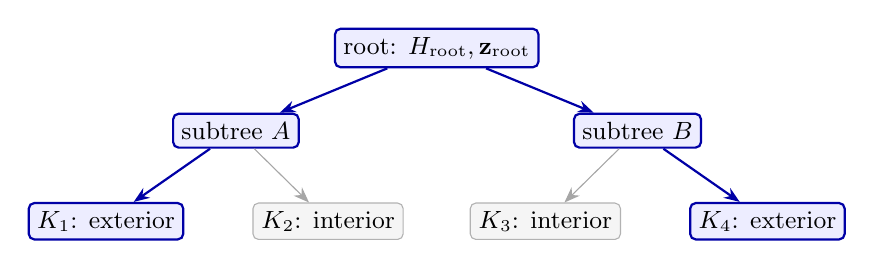
\begin{tikzpicture}[
  every node/.style={draw,rounded corners=2pt,inner sep=3pt,font=\small},
  active/.style={draw=blue!65!black,fill=blue!7,thick},
  inactive/.style={draw=gray!60,fill=gray!8}]
  \node[active] (root) at (0,1.65) {root: \(H_{\rm root},\zz_{\rm root}\)};
  \node[active] (a) at (-2.55,0.6) {subtree \(A\)};
  \node[active] (b) at (2.55,0.6) {subtree \(B\)};
  \node[active] (k1) at (-4.2,-0.55) {\(K_1\): exterior};
  \node[inactive] (k2) at (-1.38,-0.55) {\(K_2\): interior};
  \node[inactive] (k3) at (1.38,-0.55) {\(K_3\): interior};
  \node[active] (k4) at (4.2,-0.55) {\(K_4\): exterior};
  \foreach \src/\dst in {root/a,root/b,a/k1,b/k4}
    \draw[blue!65!black,thick,-{Stealth[length=2mm]}] (\src) -- (\dst);
  \foreach \src/\dst in {a/k2,b/k3}
    \draw[gray!70,-{Stealth[length=2mm]}] (\src) -- (\dst);
\end{tikzpicture}
\end{center}
\vspace{-0.4em}
\noindent\emph{Schematic:} only highlighted leaf-to-root paths carry high-flux observations. Nevertheless, a source supported in an inactive interior subtree changes its ordinary \(\bb\), hence the interface offset \(\mathbf r\) encountered on an active path, and therefore \(\zz_{\rm root}\). ``Inactive'' means \emph{no high-observation rows}, not ``irrelevant to the physical solution.''

Consequently the final root observation is
\begin{equation}\label{eq:rootH}
 \boxed{\qquad
 \mathbf q_{H,\rm root}=H_{\rm root}\lam_{\rm root}+\zz_{\rm root},\qquad
 \text{rows indexed only by global exterior high-flux modes}.\qquad}
\end{equation}
For a fixed coefficient field, \(H_{\rm root}\) is reusable across many right-hand sides. For each source update, first refresh ordinary child offsets and \(\mathbf r\) in the usual upward pass, then refresh \(\zz_N\) on active branches using \eqref{eq:propH}; no new local least-squares solves are required.

\section{Corrected root Robin equation}
Let \(M_\alpha^{LL}\) be the ordinary low-to-low face multiplication by \(\alpha\); let \(M_\beta^{LL}\) and \(M_\beta^{LH}\) be the two column blocks of the rectangular degree-\(n\) output multiplication by \(\beta\). All are block diagonal over \emph{global exterior faces}, ordered consistently with \(S_{\rm root}\), \(\bb_{\rm root}\), and \((H_{\rm root},\zz_{\rm root})\). Projecting \eqref{eq:formB} gives
\begin{align}\label{eq:rootrobinexpanded}
 \gvec
 &=M_\alpha^{LL}\lam_{\rm root}
  +M_\beta^{LL}\bigl(S_{\rm root}\lam_{\rm root}+\bb_{\rm root}\bigr)
  +M_\beta^{LH}\bigl(H_{\rm root}\lam_{\rm root}+\zz_{\rm root}\bigr).
\end{align}
Thus \emph{only the root Robin matrix and its right-hand side change}:
\begin{equation}\label{eq:rootrobinboxed}
 \boxed{\begin{aligned}
 R_{\rm root}
  &=M_\alpha^{LL}+M_\beta^{LL}S_{\rm root}
     +M_\beta^{LH}H_{\rm root},\\
 \mathbf h_{\rm root}
  &=\gvec-M_\beta^{LL}\bb_{\rm root}
     -M_\beta^{LH}\zz_{\rm root},\\
 R_{\rm root}\lam_{\rm root}&=\mathbf h_{\rm root}.
 \end{aligned}}
\end{equation}
After solving, the standard \emph{unchanged} downward pass reconstructs interfaces by \eqref{eq:gamma} and volume solutions by \eqref{eq:U}. The high flux is not used to modify merges, interface conservation, tau penalties, or the degree-\(n\) trace skeleton.

\subsection*{Sanity checks and implementation invariants}
\begin{itemize}
\item \textbf{Constant \(\beta\):} orthogonality gives \(M_\beta^{LH}=0\), recovering the validated constant-Robin equation, with no need to construct \(H_{\rm root}\).
\item \textbf{Low-degree diffusion:} if \(p_A\le1\), the physical co-normal flux has no high degree beyond \(n\). Again the correction vanishes.
\item \textbf{Zero source:} with \(\fint=0\), all \(\bb_N\), \(\mathbf r\), and \(\zz_N\) vanish. The new term is then purely \(M_\beta^{LH}H_{\rm root}\).
\item \textbf{Nonzero source:} retain the \(M_\beta^{LH}\zz_{\rm root}\) term. Neglecting it breaks the affine particular-solution contribution even if the operator correction is correct.
\item \textbf{Full numerical flux:} multiply the \emph{low augmented flux} and the \emph{high physical flux}; do not apply \(\beta\) only after truncating the physical flux, and do not introduce an additional high-order tau penalty.
\item \textbf{Face conventions:} use the common canonical face \(\kappa\), correct orientation permutations, and exactly one physical face scaling. Ensure both \(M_\beta^{LL}\) and \(M_\beta^{LH}\) derive from one correctly quadrature-resolved rectangular multiplication operator.
\item \textbf{Backend scope:} implement and validate this on the \texttt{Dense} leaf path only. Reject unsupported \texttt{DenseSparse}, \texttt{MatrixFree}, and \texttt{Verify} divergence/high-flux configurations in the public interface.
\end{itemize}

\paragraph{Minimal implementation sequence.}
(1) Assemble rectangular high physical co-normal face maps and compare with independent weighted face quadrature; (2) form leaf \(H_K\) and \(\zz_K\) on global boundary faces; (3) reuse each merge's existing \(R_A,R_B\) and source offset \(\mathbf r\) to propagate \eqref{eq:propH} only on \(\mathcal A\); (4) assemble \(M_\beta^{n\leftarrow p_H}\), extract its low/high column blocks, and solve \eqref{eq:rootrobinboxed}; (5) validate variable Robin polynomial manufactured solutions, then nonhomogeneous and convergence cases. These steps preserve the current Dense HPS interfaces and source-reuse architecture.

\end{document}
